\documentclass[12pt,letterpaper]{article}
\usepackage{graphicx,textcomp}
\usepackage{natbib}
\usepackage{setspace}
\usepackage{fullpage}
\usepackage{color}
\usepackage[reqno]{amsmath}
\usepackage{amsthm}
\usepackage{fancyvrb}
\usepackage{amssymb,enumerate}
\usepackage[all]{xy}
\usepackage{endnotes}
\usepackage{lscape}
\newtheorem{com}{Comment}
\usepackage{float}
\usepackage{hyperref}
\newtheorem{lem} {Lemma}
\newtheorem{prop}{Proposition}
\newtheorem{thm}{Theorem}
\newtheorem{defn}{Definition}
\newtheorem{cor}{Corollary}
\newtheorem{obs}{Observation}
\usepackage[compact]{titlesec}
\usepackage{dcolumn}
\usepackage{tikz}
\usetikzlibrary{arrows}
\usepackage{multirow}
\usepackage{xcolor}
\newcolumntype{.}{D{.}{.}{-1}}
\newcolumntype{d}[1]{D{.}{.}{#1}}
\definecolor{light-gray}{gray}{0.65}
\usepackage{url}
\usepackage{listings}
\usepackage{color}

\definecolor{codegreen}{rgb}{0,0.6,0}
\definecolor{codegray}{rgb}{0.5,0.5,0.5}
\definecolor{codepurple}{rgb}{0.58,0,0.82}
\definecolor{backcolour}{rgb}{0.95,0.95,0.92}

\lstdefinestyle{mystyle}{
	backgroundcolor=\color{backcolour},   
	commentstyle=\color{codegreen},
	keywordstyle=\color{magenta},
	numberstyle=\tiny\color{codegray},
	stringstyle=\color{codepurple},
	basicstyle=\footnotesize,
	breakatwhitespace=false,         
	breaklines=true,                 
	captionpos=b,                    
	keepspaces=true,                 
	numbers=left,                    
	numbersep=5pt,                  
	showspaces=false,                
	showstringspaces=false,
	showtabs=false,                  
	tabsize=2
}
\lstset{style=mystyle}
\newcommand{\Sref}[1]{Section~\ref{#1}}
\newtheorem{hyp}{Hypothesis}

\title{Problem Set 1}
\date{Due: October 1, 2021}
\author{Applied Stats/Quant Methods 1}

\begin{document}
	\maketitle
	
	\section*{Instructions}
	\begin{itemize}
		\item Please show your work! You may lose points by simply writing in the answer. If the problem requires you to execute commands in \texttt{R}, please include the code you used to get your answers. Please also include the \texttt{.R} file that contains your code. If you are not sure if work needs to be shown for a particular problem, please ask.
		\item Your homework should be submitted electronically on GitHub in \texttt{.pdf} form.
		\item This problem set is due before 8:00 on Friday October 1, 2021. No late assignments will be accepted.
		\item Total available points for this homework is 100.
	\end{itemize}
	
	\vspace{1cm}
	\section*{Question 1 (50 points): Education}

A school counselor was curious about the average of IQ of the students in her school and took a random sample of 25 students' IQ scores. The following is the data set:\\
\vspace{.5cm}

\lstinputlisting[language=R, firstline=40, lastline=43]{PS01.R}  

\vspace{1cm}

\begin{enumerate}
	\item Find a 90\% confidence interval for the average student IQ in the school.\\
	
	Answer:
	\lstinputlisting[language=R, firstline=49, lastline=57]{PS01.R}
	
	Confidence interval for the average student IQ: lower Limit= 93.96, Upper Limit = 102.92
	
	\item Next, the school counselor was curious  whether  the average student IQ in her school is higher than the average IQ score (100) among all the schools in the country.\\ 
	
	
	\noindent Using the same sample, conduct the appropriate hypothesis test with $\alpha=0.05$.
	
	Step 1: Assumptions: 
	        the type of data is quantitative data; the sample is generated by random sampling; the population is distributed normally.  
	           
	Step 2: state hypothesis:  
	        Null hypothesis: the average student IQ in the school is lower than or equal to the average IQ score (100), (H0 ≤ 100) \\
	        Alternative hypothesis: Ha > 100   \\
	        \lstinputlisting[language=R, firstline=85, lastline=90]{PS01.R}
	Step 3: Calculate a test statistics:
	 
	        \lstinputlisting[language=R, firstline=94, lastline=95]{PS01.R}
	        report TS = -0.1191488 
	        
	Step 4: P-value: 
	        \lstinputlisting[language=R, firstline=101, lastline=104]{PS01.R}
	        Report P-value = 0.72, larger than  0.05 \\
	        or
	        \lstinputlisting[language=R, firstline=108, lastline=108]{PS01.R}
	         Report P-value = 0.72, larger than 0.05 \\         
    Step 5: Draw a conclusion \\     
	        The p-value is higher than 0.05, so we cannot deny the null hypothesis that the average IQ of students in this school is lower than or equal to the average IQ of students in all schools in this country.
	        
	
	
	
	
	
\end{enumerate}

\newpage

	\section*{Question 2 (50 points): Political Economy}

\noindent Researchers are curious about what affects the amount of money communities spend on addressing homelessness. The following variables constitute our data set about social welfare expenditures in the USA. \\
\vspace{.5cm}


\begin{tabular}{r|l}
	\texttt{State} &\emph{50 states in US} \\
	\texttt{Y} & \emph{per capita expenditure on shelters/housing assistance in state}\\
	\texttt{X1} &\emph{per capita personal income in state} \\
	\texttt{X2} &  \emph{Number of residents per 100,000 that are "financially insecure" in state}\\
	\texttt{X3} &  \emph{Number of people per thousand residing in urban areas in state} \\
	\texttt{Region} &  \emph{1=Northeast, 2= North Central, 3= South, 4=West} \\
\end{tabular}

\vspace{.5cm}
\noindent Explore the \texttt{expenditure} data set and import data into \texttt{R}.
\vspace{.5cm}
\lstinputlisting[language=R, firstline=120, lastline=152]{PS01.R}  
\vspace{.5cm}
\begin{itemize}

\item
Please plot the relationships among \emph{Y}, \emph{X1}, \emph{X2}, and \emph{X3}? What are the correlations among them (you just need to describe the graph and the relationships among them)?

\lstinputlisting[language=R, firstline=159, lastline=165]{PS01.R} 

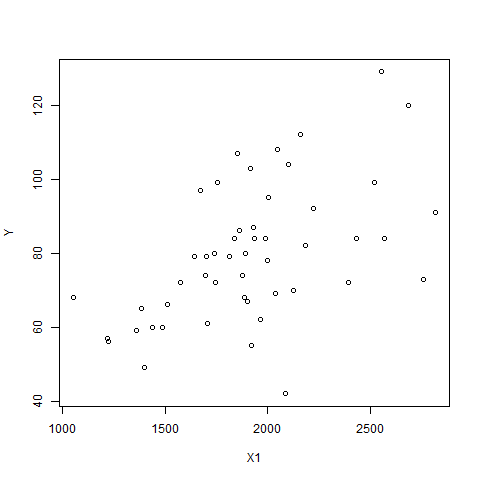
\includegraphics[scale=.80]{Y ~ X1.png}

Preliminary analysis of the graph: When X1 increases, we expect to see an increase in Y at the same time.
The coefficient of X1 is 0.025, the intercept is 32.546, which means when X1, per capita personal income in state increases by 1 US dollar, we expect to see an increase in Y, per capita expenditure on shelters/housing assistance in state, by 0.025 US dollar; When per capita personal income in state is 0 dollar, the per capita expenditure on shelters/housing assistance in state is 32.546 US dollar.
The p value of the coefficient of X1 is 7.08e-05, which is smaller than 0.001. Therefore, We can reject the null hypothesis that there is no correlation between Y and X1 at 0.001 level.



\lstinputlisting[language=R, firstline=176, lastline=182]{PS01.R} 

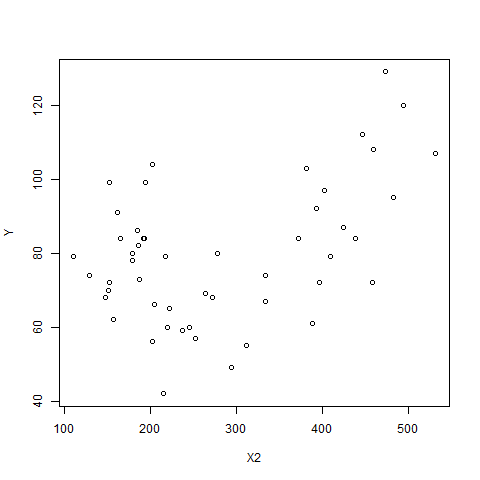
\includegraphics[scale=.80]{Y ~ X2.png}

Preliminary analysis of the graph: When X2 increases, we expect to see an increase in Y at the same time.

The coefficient of X2 is 0.070, the intercept is 59.761, which means when X2, the number of residents per 100,000 that are "financially insecure" in state increases by 1, we expect to see an increase in Y, per capita expenditure on shelters/housing assistance in state, by 0.070 US dollar; When Number of residents per 100,000 that are "financially insecure" in state is 0, the per capita expenditure on shelters/housing assistance in state is 59.761 US dollar.
The p value of the coefficient of X2 is 0.001, which is smaller than 0.01. Therefore, We can reject the null hypothesis that there is no correlation between Y and X2 at 0.01 level.



\lstinputlisting[language=R, firstline=195, lastline=201]{PS01.R} 

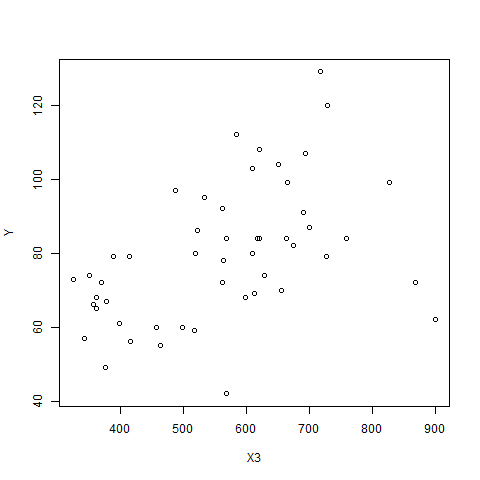
\includegraphics[scale=.80]{Y ~ X3.png}

Preliminary analysis of the graph: When X3 increases, we expect to see Y increase at the same time.

The coefficient of X3 is 0.059, the intercept is 46,306, which means when X3,the number of people per thousand residing in urban areas in state  increases by 1, we expect to see an increase in Y, per capita expenditure on shelters/housing assistance in state, by 0.059 US dollar; When Number of people per thousand residing in urban areas in state is 0, the per capita expenditure on shelters/housing assistance in state is 46.306 US dollar.
The p value of the coefficient of X3 is 0.000695, which is smaller than 0.001. Therefore, We can reject the null hypothesis that there is no correlation between Y and X3 at 0.001 level.


\lstinputlisting[language=R, firstline=214, lastline=220]{PS01.R} 

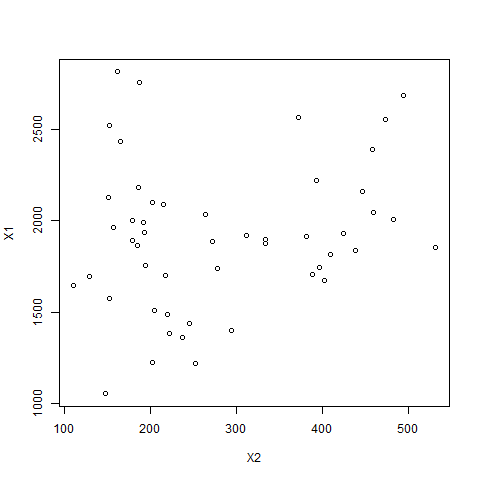
\includegraphics[scale=.80]{X1 ~ X2.png}

Preliminary analysis of the graph: there is no obvious correlation between X1 and X2.

The coefficient of X2 is 0.696, the intercept is 1715.655, which means when X2, number of residents per 100,000 that are "financially insecure" in state increases by 1, we expect to see an increase in X1, per capita personal income in state, by 0.696 US dollar; When the number of residents per 100,000 that are "financially insecure" in state is 0, the per capita personal income in state is 1715.655 US dollar.
The p value of the coefficient of X2 is 0.152, which is larger than 0.05. Therefore, We cannot reject the null hypothesis that there is no correlation between X1 and X2.



\lstinputlisting[language=R, firstline=232, lastline=238]{PS01.R} 

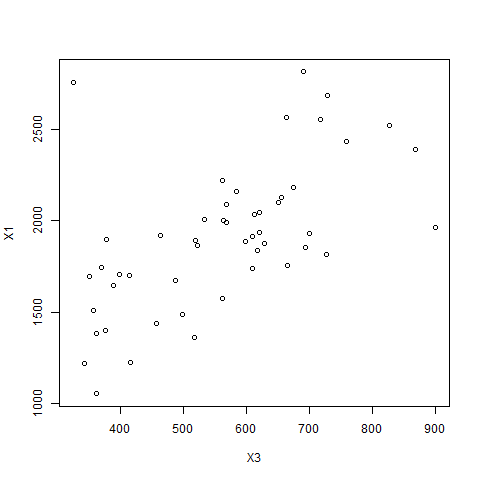
\includegraphics[scale=.80]{X1 ~ X3.png}

Preliminary analysis of the graph: when X3 increases, X1 is expected to increase at the same time.

The coefficient of X3 is 1.643, the intercept is 988.947, which means when X3, the number of people per thousand residing in urban areas in state increases by 1, we expect to see an increase in X1, per capita personal income in state, by 1.643 US dollar; When the Number of people per thousand residing in urban areas in state is 0, the per capita personal income in state is 988.947 US dollar.
The p value of the coefficient of X3 is 5.13e-06, which is smaller than 0.001. Therefore, We can reject the null hypothesis that there is no correlation between X1 and X2 at 0.001 level.



\lstinputlisting[language=R, firstline=251, lastline=257]{PS01.R} 

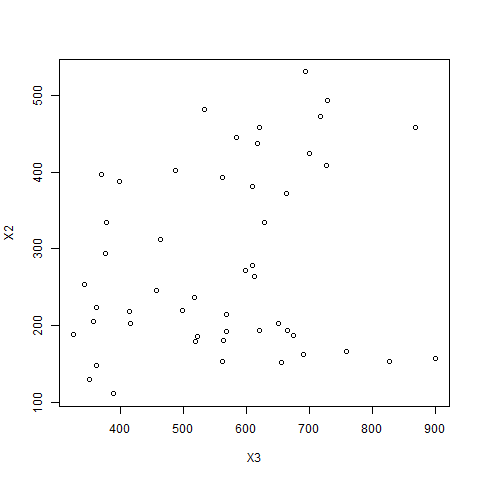
\includegraphics[scale=.80]{X2 ~ X3.png}

Preliminary analysis of the graph: There is no obvious correlation between X2 and X3. 

The coefficient of X3 is 0.180, the intercept is 180.609, which means when X3, the number of people per thousand residing in urban areas in state increases by 1, we expect to see an increase in X2, Number of residents per 100,000 that are "financially insecure" in state by 0.180; When the number of people per thousand residing in urban areas in state is 0, the number of residents per 100,000 that are "financially insecure" in state is 180.609. 
The p value of the coefficient of X3 is 0.123, which is larger than 0.05. Therefore, We cannot reject the null hypothesis that there is no correlation between X2 and X3. 



\vspace{.5cm}
\item
Please plot the relationship between \emph{Y} and \emph{Region}? On average, which region has the highest per capita expenditure on housing assistance?

\lstinputlisting[language=R, firstline=271, lastline=274]{PS01.R} 

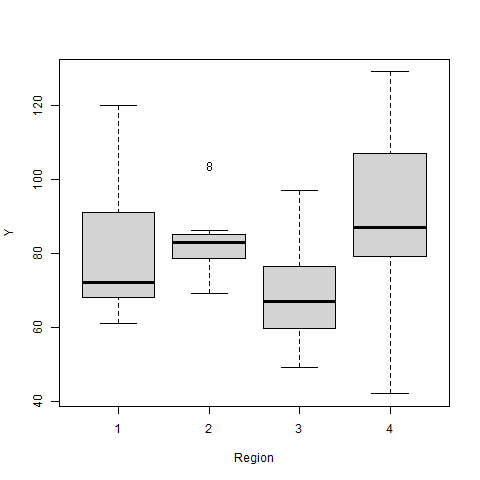
\includegraphics[scale=.80]{Y ~ Region.png}

On average, West has the highest per capita expenditure on housing assistance.



\vspace{.5cm}
\item
Please plot the relationship between \emph{Y} and \emph{X1}? Describe this graph and the relationship. Reproduce the above graph including one more variable \emph{Region} and display different regions with different types of symbols and colors.

\lstinputlisting[language=R, firstline=280, lastline=286]{PS01.R} 

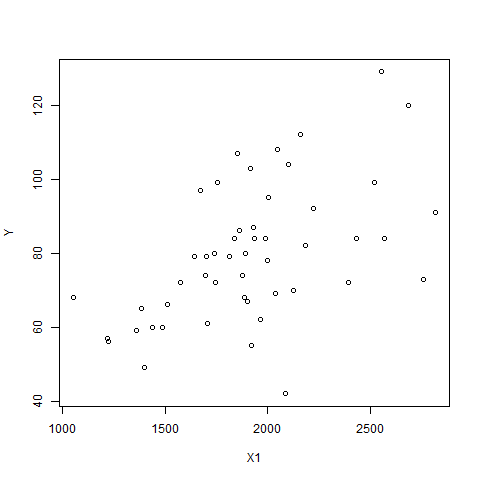
\includegraphics[scale=.80]{Y ~ X1.png}

Preliminary analysis of the graph: When X1 increases, we expect to see an increase in Y at the same time.

The coefficient of X1 is 0.025, the intercept is 32.546, which means when X1, per capita personal income in state increases by 1 US dollar, we expect to see an increase in Y, per capita expenditure on shelters/housing assistance in state, by 0.025 US dollar; When per capita personal income in state is 0 dollar, the per capita expenditure on shelters/housing assistance in state is 32.546 US dollar. 
The p value of the coefficient of X1 is 7.08e-05, which is smaller than 0.001. Therefore, We can reject the null hypothesis that there is no correlation between Y and X1 at 0.001 level.



\lstinputlisting[language=R, firstline=298, lastline=305]{PS01.R} 

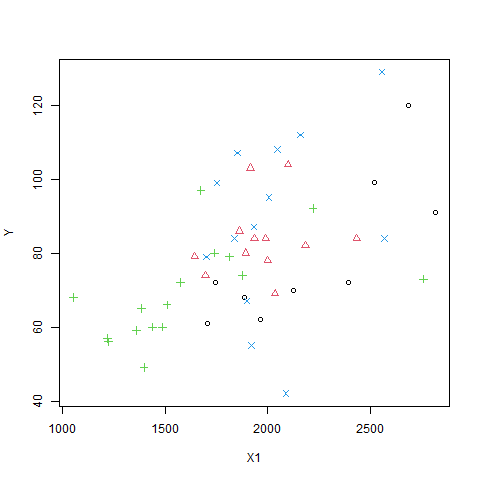
\includegraphics[scale=.80]{Y ~ X1, colour, symbol.png}

The coefficient of X1 is 0.027, the coefficient of Region is 3.333, which means when X1, per capita personal income in state increases by 1 US dollar, we expect to see an increase in Y, per capita expenditure on shelters/housing assistance in state, by 0.027 US dollar; when the region is different, we expect to see an average difference in the per capita expenditure on shelters/housing assistance in state of 3.333 US dollar. 
The p value of the coefficient of X1 is 2.77e-05, which is smaller than 0.001. Therefore, We can reject the null hypothesis that there is no correlation between Y and X1 at 0.001 level. 

The p value of the coefficient of Region is 0.128, which is larger than 0.05.
Therefore, we cannot reject the null hypothesis that there is no correlation between Y and Region.

\end{itemize}


\end{document}
